\section{Planejamento}
\begin{frame}[fragile]
%[fragile, allowframebreaks=0.9]

    \frametitle{Planejamento}

   \begin{block}{}
     \begin{itemize}
      \item Requisito: conceitos de listas e recursividade  dominados!
       \pause
      
      \item Além destes: conceitos grafos, árvores de busca, nós, etc
       
       \pause
      \item \textit{Planejamento} é um termo amplo e em vários domínios 
      
       \pause
      \item O que \textbf{não} é o nosso contexto de \textit{planejamento} ?\\
      Exemplo: planejamento estratégico das empresas, planejar como distribuir
      os dividendos da empresa, orçamento familiar,  etc
      
      \pause
      
      
      \item O que é o nosso contexto de \textit{planejamento} ?
       \pause
       Questões que envolvam um ambiente, um agente, sensores,
      e  ações que modifiquem estados.\\ Exemplo clássico:  robótica em geral
 

    \end{itemize}
    
    \end{block}
    
\end{frame}



\begin{frame}[fragile]
%[fragile, allowframebreaks=0.9]

    \frametitle{Planejamento}

   \begin{block}{}
     \begin{itemize}
 

%      \item 
      
      
 %     \pause

 
       
      \item Problemas em geral necessitam de um \textbf{plano} para serem solucionados

      \item Em resumo, a área de planejamento é bem complexa,  antiga na área da IA e robótica (1970 -- STRIPS), 
      efervescente, e de muito interesse na indústria.
      
      
      \pause
      
      \item Vários problemas ainda sem solução 
      
      \pause
      
      \item Várias abordagens sobre a visão clássica da IA. Mas temos evoluções
      significativas ...
      
      \pause
      \item PDDL (\textit{Planning Domain Definition Language}) : unanimidade (ou próxima a esta)
      entre os pesquisadores de planejamento
%      \pause
      
%     \item 

    \end{itemize}
    
    \end{block}
    
\end{frame}



\begin{frame}[fragile]
%[fragile, allowframebreaks=0.9]

  \frametitle{Definições}

   \begin{block}{}
     \begin{itemize}
      \item Plano: seqüência ordenada de ações
       \pause
         \begin{itemize}
           \item problema: obter banana, leite e uma furadeira
            \item plano: ir ao supermercado, ir à seção de frutas, pegar as bananas, ir à seção de leite, pegar uma caixa de leite, ir ao caixa,  pagar tudo, ir a uma loja de ferramentas, ..., voltar para casa.
                                
         \end{itemize}
       
       \item Um Planejador:
         
       \pause
        Combina conhecimento de um ambiente, um agente e suas ações possíveis,
        entradas (luz, cor, cheiro, sensor, etc), um estado corrente
        e/ou inicial, e com isto resolve de problemas planejar sequência
        de ações, que mudam de estados a cada ação, até atingir um 
        estado final.
       
    \end{itemize}
    
    \end{block}
    
\end{frame}



\begin{frame}[fragile]
\frametitle{Exemplos do que é planejamento ...}

\begin{figure}[!htb]
\centering
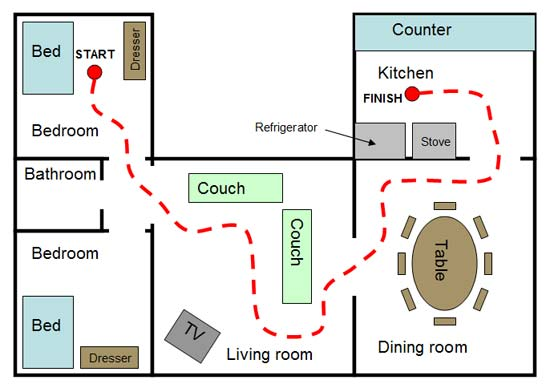
\includegraphics[width=0.60\textwidth, height=0.650\textheight]{figures/planning01.jpg}
%%%prolog/scale=0.47
%\label{fig_nos_estados}
\caption{A fome no meio da noite!}
\end{figure}

%\framebreak

\end{frame}


\begin{frame}[fragile]
\frametitle{Exemplos do que é planejamento ...}

\begin{figure}[!htb]
\centering
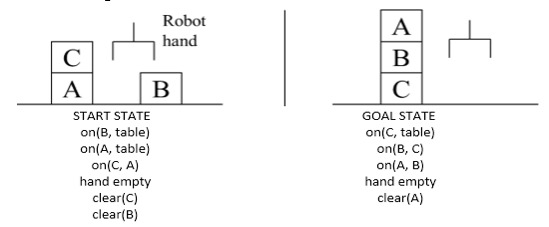
\includegraphics[width=0.850\textwidth, height=0.650\textheight]{figures/mundo_dos_blocos01.jpg}
%%%prolog/scale=0.47
%\label{fig_nos_estados}
\caption{O \textit{mundo dos blocos}}
\end{figure}

%\framebreak

\end{frame}


\begin{frame}[fragile]
\frametitle{Espaço de Estados}

\begin{figure}[!htb]
\centering
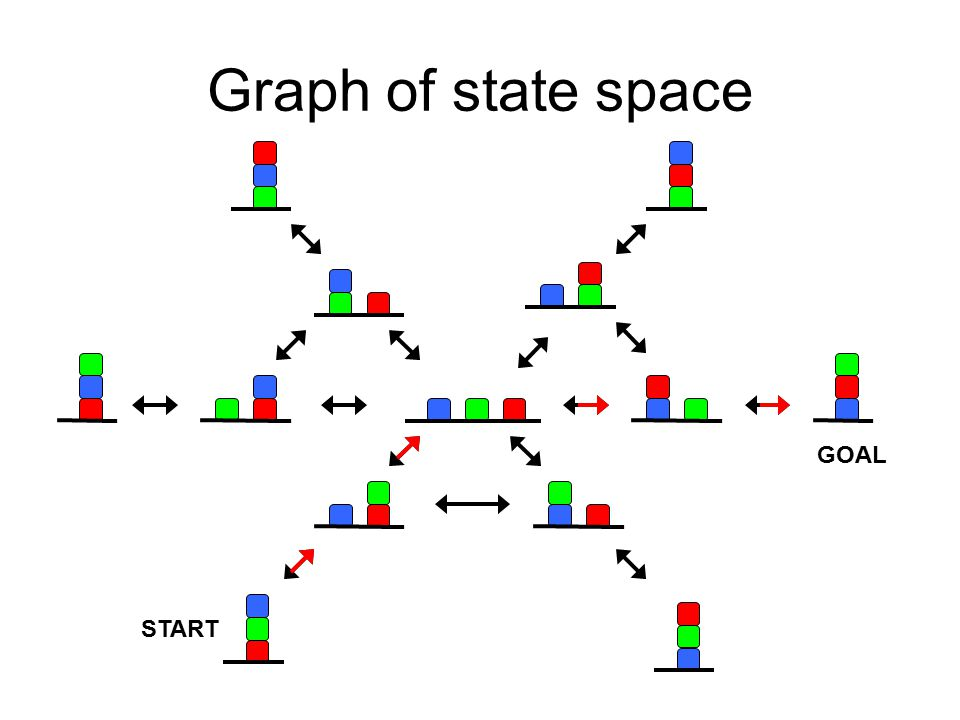
\includegraphics[width=0.7\textwidth, height=0.70\textheight]{figures/mundo_dos_blocos02.jpg}
%%%prolog/scale=0.47
%\label{fig_nos_estados}
\caption{O espaço de estados do \textit{mundo dos blocos}}
\end{figure}

%\framebreak

\end{frame}



\begin{frame}[fragile, allowframebreaks=0.9]
\frametitle{Elementos de um  Planejador -- Vocabulário}

\textcolor{red}{PAREI AQUI}

\begin{itemize}
 \item Plano: uma sequência ordenada de ações, 
 criada incrementalmente a partir do estado inicial\\
Ex. posições das peças de um jogo\\
$$S_1 < S_2 < ... < S_n$$
 
  \item Ambiente:
agente, Wumpus, cavernas, buracos, ouro

  \item  Estados:   descrição completa de possíveis estados atingíveis\\
  Problema: quanto aos estados não-previstos, inacessíveis?

  \item  Estado inicial:
agente na caverna (1,1) com apenas uma flecha
 Wumpus e buracos em cavernas quaisquer

  \item Objetivos:
pegar a barra de ouro e voltar à caverna (1,1) com vida

  \item  Percepções: 
fedor, brisa, luz, choque (contra a parede da caverna) e grito do Wumpus

  \item Ações: programas que geram o estado sucessor
avançar para próxima caverna
girar 90 graus à direita ou à esquerda
pegar um objeto na mesma caverna que o agente
atirar na direção para onde o agente está olhando (a flecha pára quando encontra uma parede ou mata o Wumpus)
 sair da caverna
 
 \item Operadores: tudo o que o agente pode fazer
 
 \item Heurística: número de objetos ainda não possuídos
 
\end{itemize}

\end{frame}




\begin{frame}[fragile, allowframebreaks=0.9]
  \frametitle{O Problema Exemplo}

\begin{figure}[!htb]
\centering
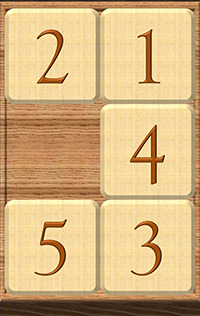
\includegraphics[width=.5\textwidth, height=0.40\textheight]{figures/puzzle_2x3_01.jpg}
%%%prolog/scale=0.47
%\label{fig_nos_estados}
\caption{Um quebra-cabeça ($2\times 3$ ou $3\times 2$) \textit{simplificado} do conhecido $3\times 3$}
\end{figure}


\framebreak
\begin{figure}[!htb]
\centering
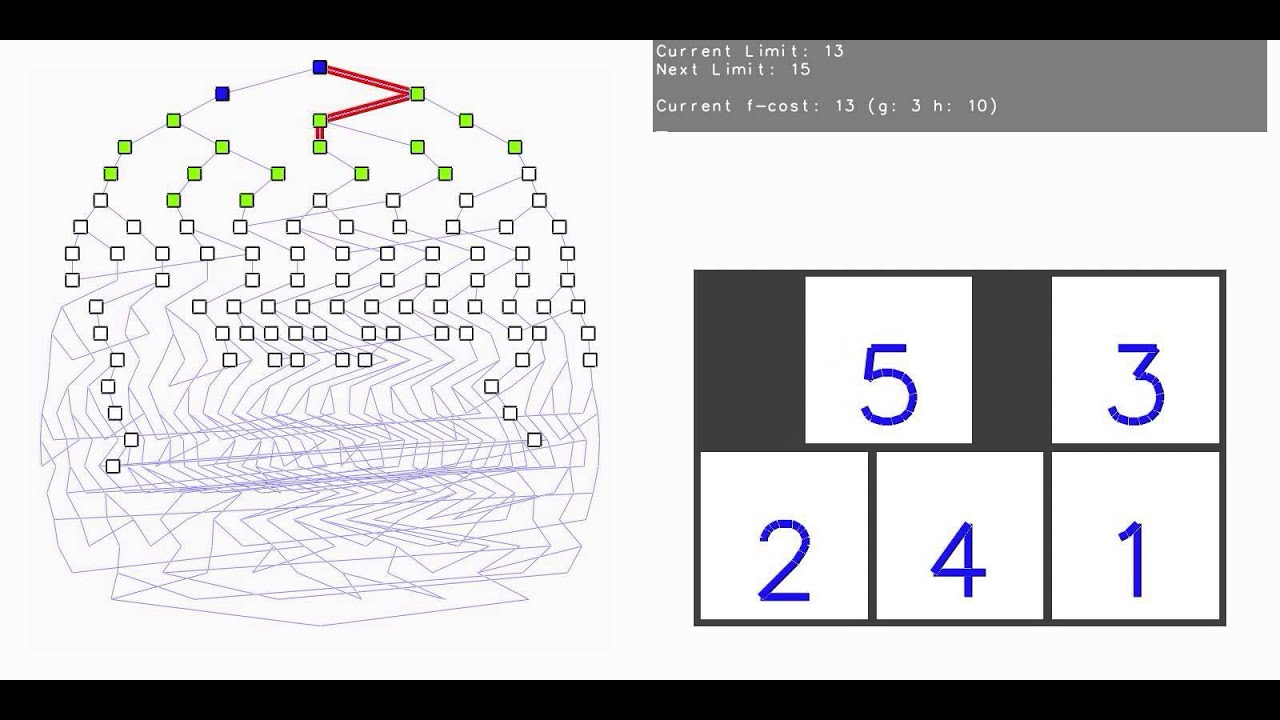
\includegraphics[width=.75\textwidth, height=0.65\textheight]{figures/puzzle_2x3_02.jpg}
%%%prolog/scale=0.47
%\label{fig_nos_estados}
\caption{Sim, \textit{simplificado} mas não muito!}
\end{figure}

\end{frame}

\begin{frame}[fragile, allowframebreaks=0.9]
 \frametitle{Partes do  código comentado}

\begin{verbatim}
/*
A  B  C 
D  E  F
*/

%%%%%%%%%
%   1 5 %
% 4 3 2 %
%%%%%%%%%

import datetime.
import planner.
\end{verbatim}
\framebreak

\begin{verbatim}
index(-)
estado_inicial( [0,1,5,4,3,2]  ).

%% funcao final do planner
final( [1,2,3,4,5,0] ) => true .


\end{verbatim}
\framebreak

\begin{verbatim}
% Up <-> Down
/* Descrevendo as possiveis acoes para o planner */
action([A,B,C, D,E,F], S1, Acao, Custo_Acao ) ?=>
    Custo_Acao = 1,
    ( A == 0 ),  %% conj. condicoes
    S1 = [D,B,C, 0,E,F], 
    Acao = ($up(D),S1). %%a acao + estado modificado

action([A,B,C, D,E,F], S1, Acao, Custo_Acao ) ?=>
    Custo_Acao = 1,
    (A == 0 ),  %% conj. condicoes
    S1 = [0,B,C, A,E,F],
    Acao = ($dow(A),S1). %%a acao + estado modificado
.........................................................
\end{verbatim}
\framebreak


\begin{verbatim}
% Left <-> Right
action([A,B,C, D,E,F], S1, Acao, Custo_Acao ) ?=>
    Custo_Acao = 1,
    (A == 0),  %% conj. condicoes
    S1 = [B,0,C, D,E,F],
    Acao = ($left(B), S1). %%a acao + estado modificado
    
action([A,B,C, D,E,F], S1, Acao, Custo_Acao ) ?=>
    Custo_Acao = 1,
    (B == 0),  %% conj. condicoes
    S1 = [0,A,C, D,E,F],
    Acao = ($right(A), S1). %%a acao + estado modificado
.........................................................
\end{verbatim}

\framebreak

\begin{small}
\begin{verbatim}
main  ?=>  
    estado_inicial( Q ),
   
    best_plan_unbounded( Q , Sol_Acoes), 
     println(sol=Sol_Acoes),
        
    printf("\n Estado Inicial: "),
    w_Quadro( Q ), 
    w_L_Estado( Sol_Acoes ), 
  
    Total := length(Sol_Acoes) ,
    Num_Movts := (Total -1) ,
    printf("\n Inicial  (estado): %w ", Q),
    printf("\n Total de acoes: %d", Total), 
    printf(" \n =========================================\n ")
    %%% , fail descomente para multiplas solucoes
    .
   
main => printf("\n Para uma solução .... !!!!" ) .
.........................................................
\end{verbatim}

\end{small}

\end{frame}



\begin{frame}[fragile]
 \frametitle{O código}

\begin{itemize}
  \item Acompanhar as explicações do código de:\\
\url{https://github.com/claudiosa/CCS/blob/master/picat/puzzle_2x3_planner.pi}

  \item Confira a execuç\~ao
\end{itemize}
\end{frame}


\begin{frame}[fragile, allowframebreaks=0.9]
 \frametitle{Parte da Saída}

\begin{small}
\begin{verbatim}
[ccs@gerzat picat]$ picat puzzle_2x3_planner.pi 
sol = [(left(1),[1,0,5,4,3,2]),(left(5),[1,5,0,4,3,2]),
(up(2),[1,5,2,4,3,0]),(right(3),[1,5,2,4,0,3]),(dow(5),[1,0,2,4,5,3]),
(left(2),[1,2,0,4,5,3]),(up(3),[1,2,3,4,5,0])]

 Estado Inicial: 
 0 1 5
 4 3 2

Acao: left(1)
 1 0 5
 4 3 2

Acao: left(5)
 1 5 0
 4 3 2
.................................
\end{verbatim}
\end{small}

\framebreak
\begin{small}
\begin{verbatim}
.................................
Acao: left(2)
 1 2 0
 4 5 3

Acao: up(3)
 1 2 3
 4 5 0

 Inicial  (estado): [0,1,5,4,3,2] 
 Total de acoes: 7 
 =========================================

\end{verbatim}
\end{small}

\end{frame}



\begin{frame}[fragile]
 \frametitle{O módulo do \textit{planner} do Picat}

\begin{itemize}
  \item O que efetivamente voce precisa saber
  \pause
  \item Importar um módulo 
  \pause
  \item O predicado \textit{final}
    \pause
  \item O predicado \textit{action}
    \pause
  \item Os planejadores disponíveis: 
\end{itemize}
\end{frame}




\begin{frame}[fragile]
\frametitle{Uma Soluç\~ao -- Saída}

\begin{figure}[!htb]
\centering
%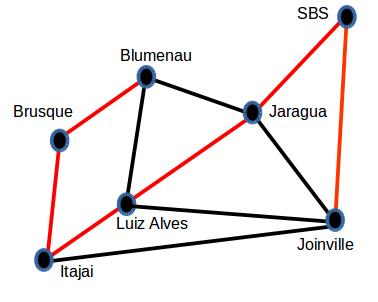
\includegraphics[width=.8\textwidth, height=0.567\textheight]{figures/mapa02SC.jpg}
%%%prolog/scale=0.47
%\label{fig_nos_estados}
%\caption{Mapa do norte de Santa Catarina}
\end{figure}

\end{frame}


\begin{frame}[fragile]
\frametitle{Reflexões}


\begin{itemize}
  \item Outros métodos para se resolver estes problemas
  \pause
  \item Mas perdemos na portabilidade de usar em outros planejadores
  \pause
  \item Os modelos escritos em PDDL (\textit{Planning Domain Definition Language})
  facilmente portáveis para Picat
    \pause
  \item Sob um uso mais restrito, um modelo em PDDL é executado diretamente em Picat
    \pause
  \item 
\end{itemize}

\end{frame}






